\documentclass{beamer}
\usepackage{graphicx}
\graphicspath{ {./images/} }

% \usepackage{beamerthemesplit} // Activate for custom appearance

\title{Differential Equations}
\subtitle{Team 6}

\author{Miguel McPherson\\ Bindu Ponugoti\\ Simrat Nijjer\\ Devyn Kipphut }
\date{Feb 25 2021}

\begin{document}

\frame{\titlepage}

\begin{frame}[allowframebreaks]
  \frametitle {Introduction}
  \begin{figure}
    \begin{minipage}{.65\textwidth}
      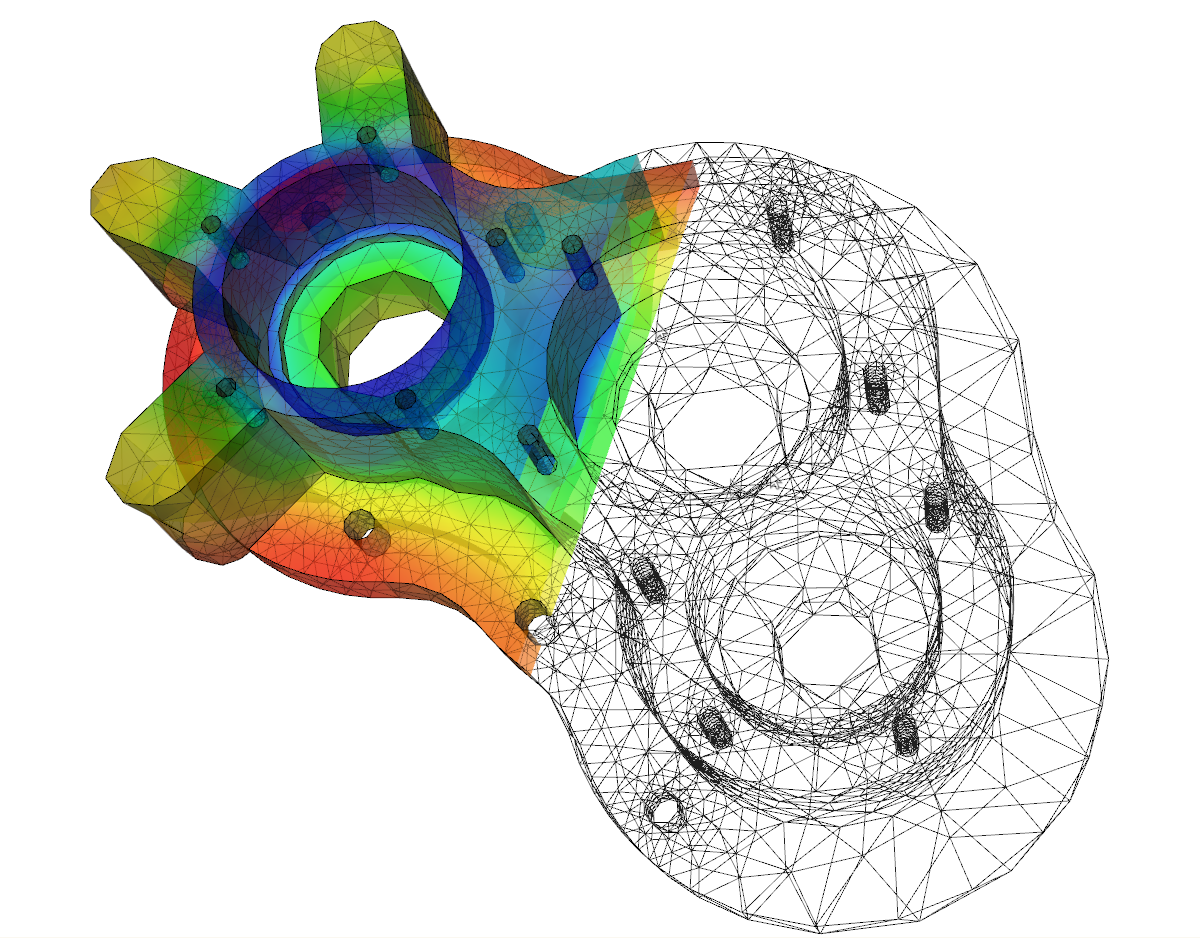
\includegraphics[width=\linewidth]{differentialEquationsIntroimage1} 
      \caption{Visualization of heat transfer in a pump casing, created by solving the heat equation. Heat is being generated internally in the casing and being cooled at the boundary, providing a steady state temperature distribution.}
    \end{minipage}\hfill
  \end{figure}
\end{frame}

\begin{frame}[allowframebreaks]
\frametitle {Introduction}
    In mathematics, a differential equation is an equation that relates on or more functions and their derivatives.
    In applications, the functions generally represent physical quantities, the derivatives represent their rates of change,
    and the differential equation defines a relationship between the two. Such relations are common; therefore, differential equations play a prominent role in 
    many disciplines including engineering, physics, economics, and biology. 
    \\~\\
    Mainly the study of differential equations consists of the study of their solutions (the set of functions that satisfy each equation), and of the properties fo their solutions.
    Only the simplest differential equations are solvable by explicit formulas; however, many properteis of solutions of a given differential equation may be determined without
    computing them exactly. 
    \\\framebreak
    Often when a closed-form expression for the solutions is not available, solutions may be approximated numerically using computers. 
    The theory of dynamical systems puts emphasis on qualitative analysis of systems described by differential equations, 
    while many numerical methods have been developed to determine solutions with a given degree of accuracy.
\end{frame}

\begin{frame}[allowframebreaks]
  \frametitle {History}
  \begin{figure}
    \begin{minipage}{.45\textwidth}
      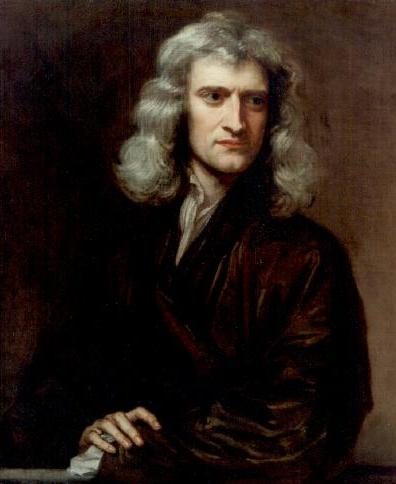
\includegraphics[width=\linewidth]{historyNewton} 
      \caption{Issac Newton}
    \end{minipage}\hfill
    \begin{minipage}{.45\textwidth}
      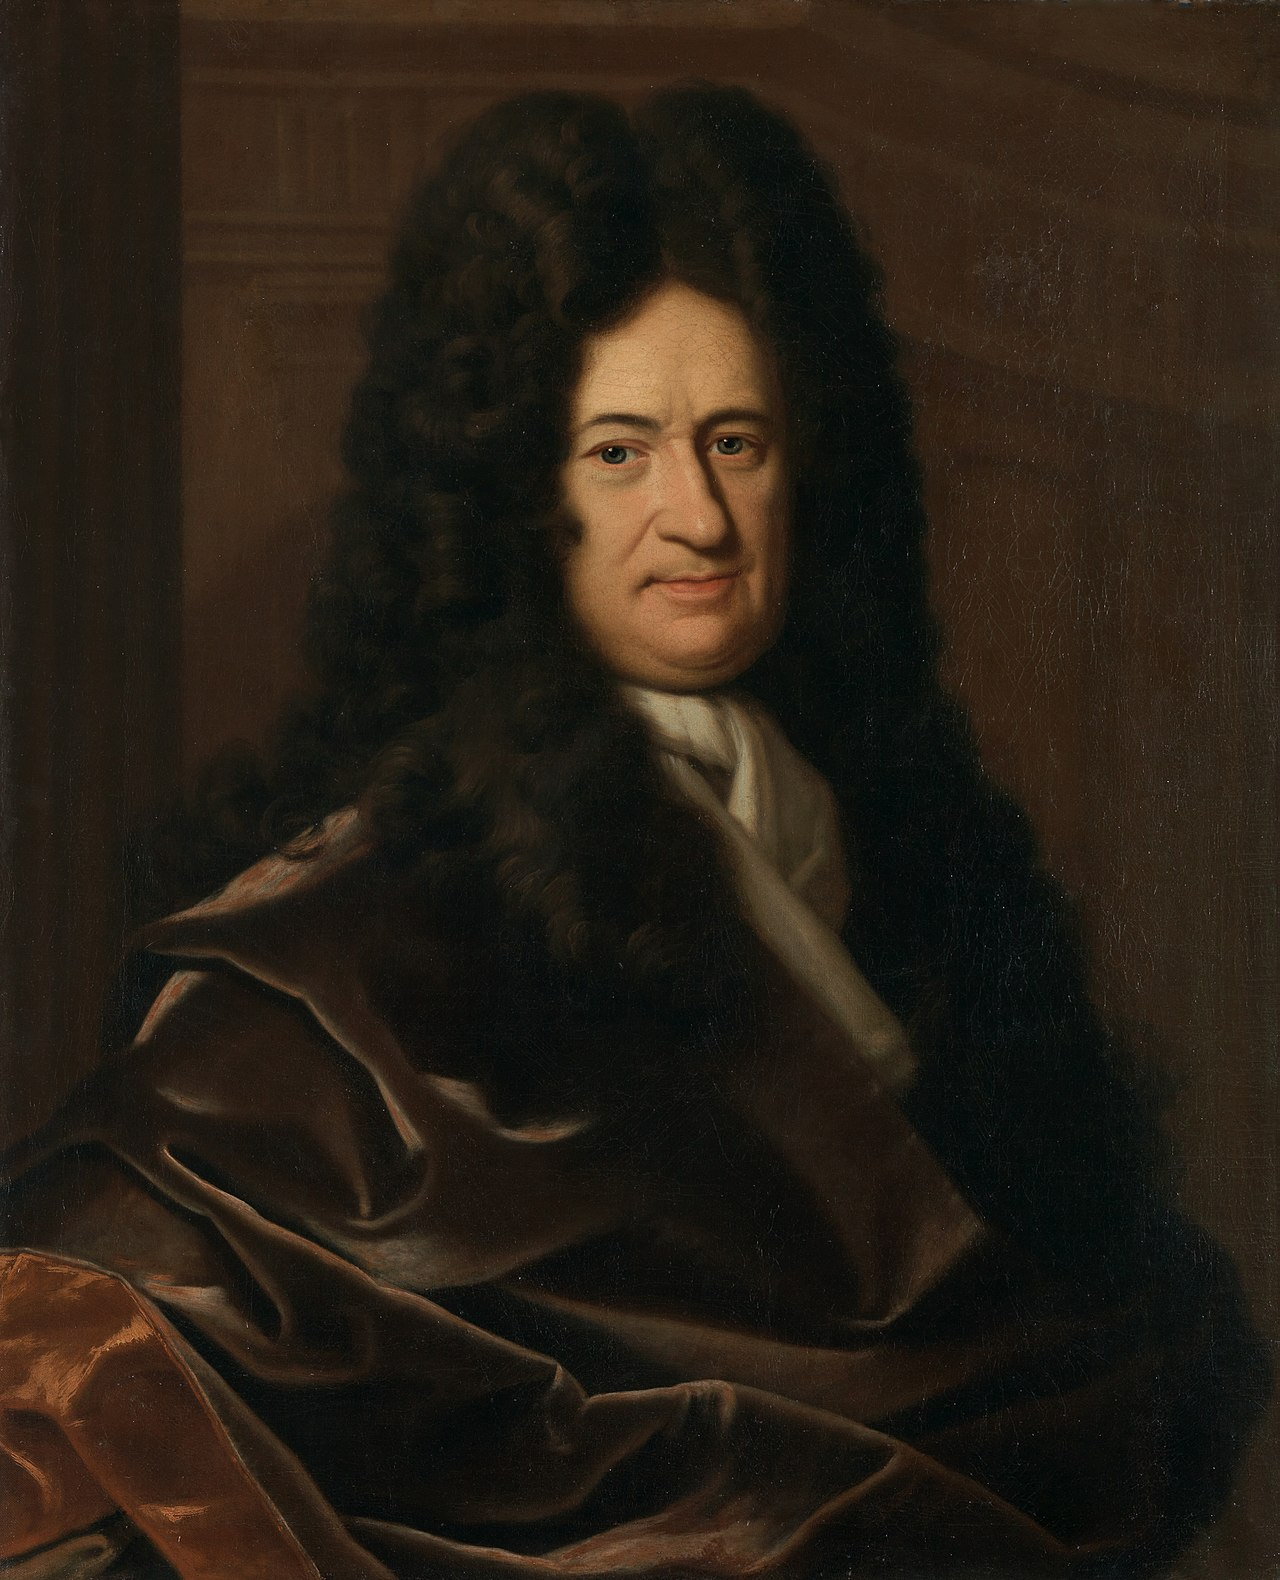
\includegraphics[width=\linewidth]{leibniz}
      \caption{Leibniz}
    \end{minipage}
  \end{figure}
\end{frame}

\begin{frame}[allowframebreaks]
\frametitle {History}
  Differential equations first came into existence with the invention of calculus by Newton and Leibniz. 
  In Chapter 2 of his 1671 work Methodus fluxionum et Serierum Infinitarum,[2] Isaac Newton listed three kinds of differential equations:
  \[{\frac{dy}{dx}}=f(x)\]
  \[{\frac{dy}{dx}}=f(x,y)\]
  \[{x_1\frac{dy}{dx_1}} + {x_2\frac{dy}{dx_2}}=y\]
  \\\framebreak
  In all these cases, y is an unknown function of x (or of x1 and x2), and f is a given function.
  He solves these examples and others using infinite series and discusses the non-uniqueness of solutions.
  Jacob Bernoulli proposed the Bernoulli differential equation in 1695.[3] This is an ordinary differential equation of the form
\end{frame}

\begin{frame}[allowframebreaks]
\frametitle {Example}
  In classical mechanics, the motion of a body is described by its position and velocity as the time value varies. 
  Newton's laws allow these variables to be expressed dynamically (given the position, velocity, acceleration and various forces acting on the body) 
  as a differential equation for the unknown position of the body as a function of time.
  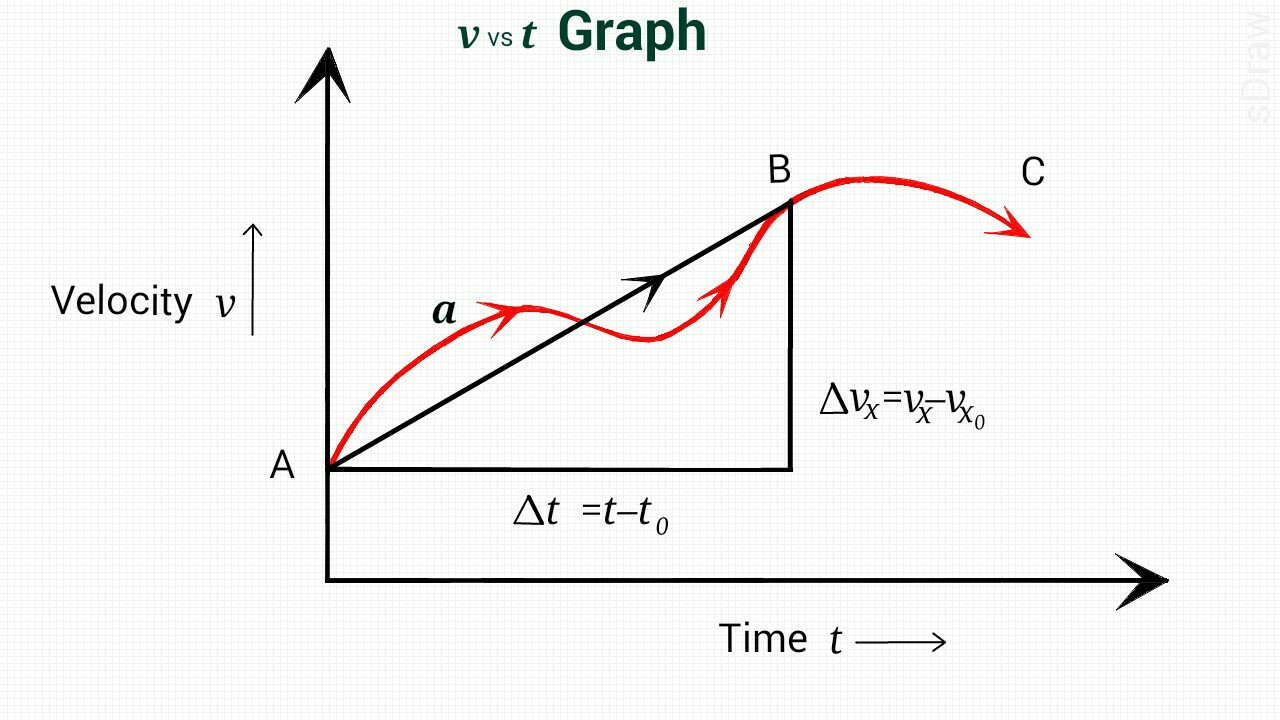
\includegraphics[width=.7\linewidth]{equationOfMotion}
  In some cases, this differential equation (called an equation of motion) may be solved explicitly.
  \\\framebreak
  An example of modeling a real-world problem using differential equations is the determination of the velocity of a ball falling through the air, considering only gravity and air resistance. 
  The ball's acceleration towards the ground is the acceleration due to gravity minus the deceleration due to air resistance. Gravity is considered constant, and air resistance may be modeled as proportional to the ball's velocity. 
  This means that the ball's acceleration, which is a derivative of its velocity, depends on the velocity (and the velocity depends on time). Finding the velocity as a function of time involves solving a differential equation and verifying its validity.

\end{frame}

\begin{frame}[allowframebreaks]
\frametitle {Types}
  Differential equations can be divided into several types. Apart from describing the properties of the equation itself, these classes of differential equations can help inform the choice of approach to a solution. 
  Commonly used distinctions include whether the equation is ordinary or partial, linear or non-linear, and homogeneous or heterogeneous. This list is far from exhaustive; 
  there are many other properties and subclasses of differential equations which can be very useful in specific contexts.

  \begin{itemize}
    \item Ordinary differential equations.
    \item Partial differential equations.
    \item Non-linear differential equations.
    \item Equation order.      
    \end{itemize}
\end{frame}

\begin{frame}
  \frametitle {Types - Ordinary differential equations}
  An ordinary differential equation (ODE) is an equation containing an unknown function of one real or complex variable x, its derivatives, and some given functions of x. 
  The unknown function is generally represented by a variable (often denoted y), which, therefore, depends on x. Thus x is often called the independent variable of the equation. 
  The term "ordinary" is used in contrast with the term partial differential equation, which may be with respect to more than one independent variable.
  \end{frame}

  \begin{frame}
  \frametitle {Types - Partial differential equations}
  A partial differential equation (PDE) is a differential equation that contains unknown multivariable functions and their partial derivatives. 
  (This is in contrast to ordinary differential equations, which deal with functions of a single variable and their derivatives.) 
  PDEs are used to formulate problems involving functions of several variables, and are either solved in closed form, or used to create a relevant computer model.
  \end{frame}

  \begin{frame}
  \frametitle {Types - Non-linear differential equations}
  A non-linear differential equation is a differential equation that is not a linear equation in the unknown function and its derivatives 
  (the linearity or non-linearity in the arguments of the function are not considered here). There are very few methods of solving nonlinear differential equations exactly; 
  those that are known typically depend on the equation having particular symmetries. Nonlinear differential equations can exhibit very complicated behaviour over extended time intervals, characteristic of chaos. 
  Even the fundamental questions of existence, uniqueness, and extendability of solutions for nonlinear differential equations, and well-posedness of initial and boundary value problems for nonlinear 
  PDEs are hard problems and their resolution in special cases is considered to be a significant advance in the mathematical theory (cf. Navier–Stokes existence and smoothness). 
  However, if the differential equation is a correctly formulated representation of a meaningful physical process, then one expects it to have a solution.
  \end{frame}

  \begin{frame}
  \frametitle {Types - Equation order}
  Differential equations are described by their order, determined by the term with the highest derivatives. 
  An equation containing only first derivatives is a first-order differential equation, an equation containing the second derivative is a second-order differential equation, and so on. 
  Differential equations that describe natural phenomena almost always have only first and second order derivatives in them, but there are some exceptions, 
  such as the thin film equation, which is a fourth order partial differential equation.
  \end{frame}

\begin{frame}[allowframebreaks]
  \frametitle {Conclusion - Applications}
  \begin{figure}
    \begin{minipage}{.45\textwidth}
      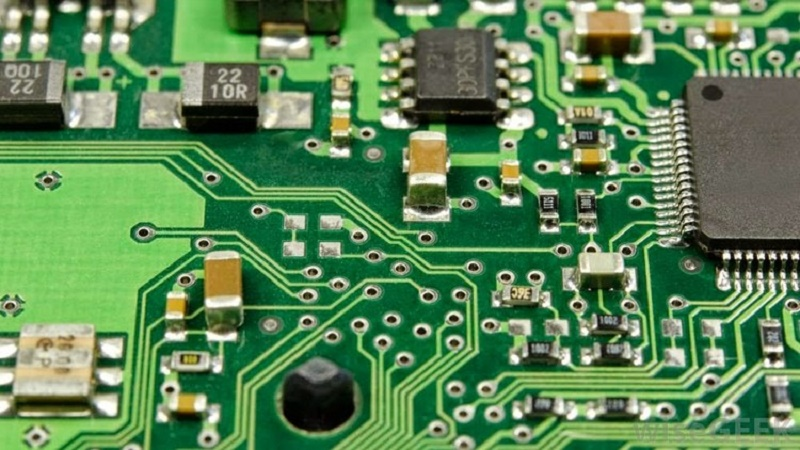
\includegraphics[width=\linewidth]{electricCircuit} 
      \caption{Electric Circuit}
    \end{minipage}\hfill
    \begin{minipage}{.45\textwidth}
      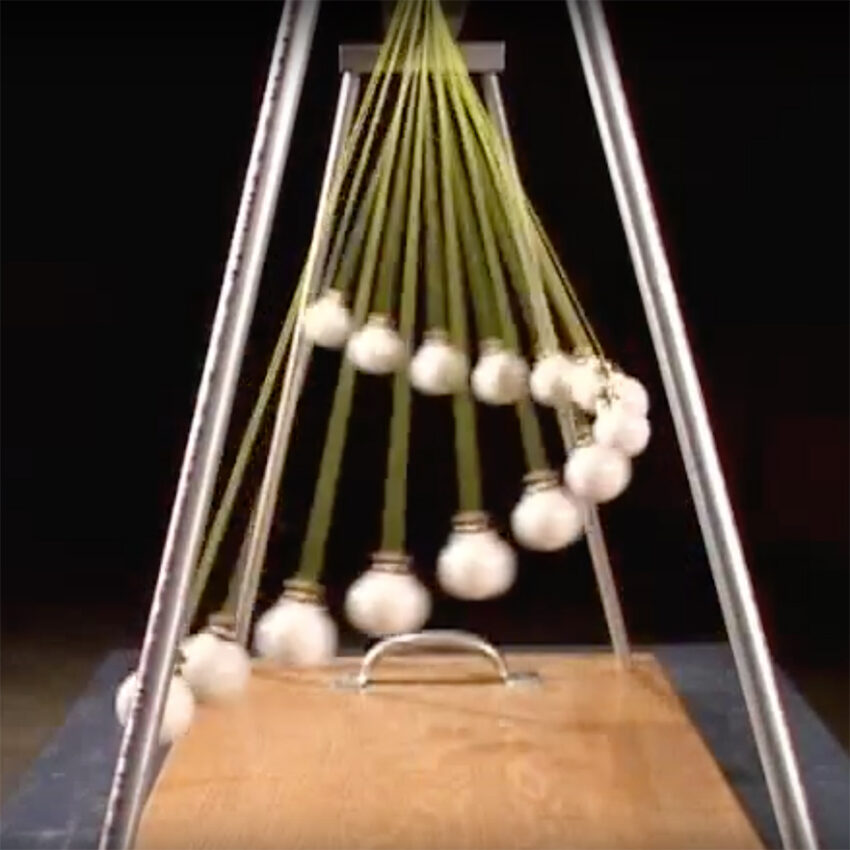
\includegraphics[width=\linewidth]{pendulummovement}
      \caption{movement - pendulum}
    \end{minipage}
    \begin{minipage}{.45\textwidth}
      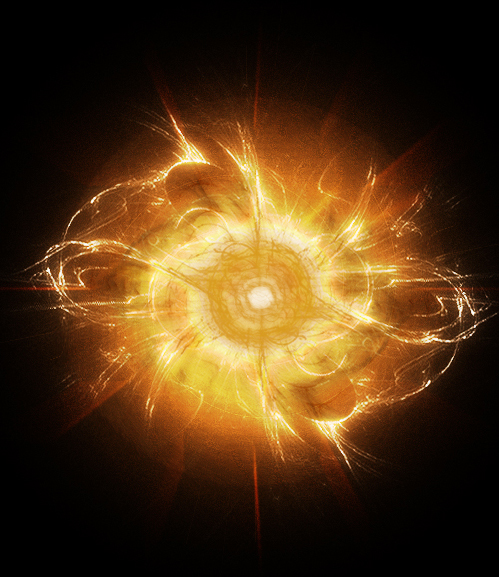
\includegraphics[width=\linewidth]{thermodynamics}
      \caption{thermodynamics}
    \end{minipage}
  \end{figure}
\end{frame}

\begin{frame}
\frametitle {Conclusion - Applications}
  The study of differential equations is a wide field in pure and applied mathematics, physics, and engineering. All of these disciplines are concerned with the properties of differential equations of various types. 
  Pure mathematics focuses on the existence and uniqueness of solutions, while applied mathematics emphasizes the rigorous justification of the methods for approximating solutions. 
  Differential equations play an important role in modeling virtually every physical, technical, or biological process, from celestial motion, to bridge design, to interactions between neurons. 
  Differential equations such as those used to solve real-life problems may not necessarily be directly solvable, i.e. do not have closed form solutions. Instead, solutions can be approximated using numerical methods.
\end{frame}

\end{document}
